\section[Theory]{Vector fitting}
\begin{frame}
	\frametitle{Vector fitting basics}
	\begin{columns}[c]
		\column{0.5\textwidth}
			\begin{itemize}
				\item<1-> Vector fitting fits a transfer function to measured input and output data
				\item<2-> Finding the parameters in~\eqref{eq:VFBasic} is a nonlinear optimization.
				\item<3-> The idea behind vector fitting presented in~\cite{gustavsen_rational_1999} is to formulate the augmented problem~\eqref{eq:VFAug} with known poles $\tilde{p_i}$.
			\end{itemize}
		\column{0.5\textwidth}
			\begin{itemize}
					\item[]<1->
				\begin{equation}
					Y(s) = H(s)\cdot U(s)
				\end{equation}
			\item[]<2-> 
				\begin{equation}
					\label{eq:VFBasic}
					H(s) = d + \sum^{n_p}_{i=1}\frac{r_i}{s-p_i}
				\end{equation}
			\item[]<3->
				\begin{equation}
					\label{eq:VFAug}
					\sigma(s)H(s) = d + \sum^{n_p}_{i=1}\frac{r_i}{s-\tilde{p_i}}
				\end{equation}
			\end{itemize}
	\end{columns}
\end{frame}
\begin{frame}
	\frametitle{Vector fitting basics continued}
	\begin{columns}[c]
		\column{0.35\textwidth}
		\begin{itemize}
				\item<1-> How do we choose $\sigma(s)$?
				\item<2-> First rewrite~\eqref{eq:VFBasic} and~\eqref{eq:VFAug}.
				\item<3-> We can see that the zeros of $\sigma(s)$ must cancel the poles of~\eqref{eq:VFBasic_prod}
		\end{itemize}
		\column{0.65\textwidth}
			\begin{itemize}
				\item[]<2->
					\begin{equation}
						\label{eq:VFBasic_prod}
						H(s) = \frac{\prod_{i=1}^{n_z}(1-z_i)}{\prod_{i=1}^{n_p}(1-p_i)}
					\end{equation}
					\begin{equation}
						\label{eq:VFAug}
						\sigma(s)H(s) = \frac{\prod_{i=1}^{n_z}(1-z_i)}{\prod_{i=1}^{n_p}(1-\tilde{p_i})}
					\end{equation}
				\item[]<3->
					\begin{equation}
						\label{eq:VFWeight}
						\sigma(s) = \frac{\prod_{i=1}^{n_z}(1-\tilde{z_i})}{\prod_{i=1}^{n_p}(1-\tilde{p}_i)}
					\end{equation}
			\end{itemize}
		\end{columns}
	\end{frame}

\begin{frame}
	\setcounter{equation}{2}
	\frametitle{Vector fitting basics continued}
	\begin{columns}[c]
		\column{0.35\textwidth}
			\begin{itemize}
				\item<1-> \eqref{eq:VFAug} can now be solved by measuring $H(s)$ at multiple frequencies and multiplying with~\eqref{eq:VFWeight} which gives~\eqref{eq:VF_prob}
				\item<2-> In~\eqref{eq:VF_prob} the unknowns are $d,r_i,k_i$ for $\tilde{p_i}$ an initial guess is used.
				\item<3-> The procedure is performed again with the calculated zeros of~\eqref{eq:VFAug} as the updated starting poles $\tilde{p_i}$
			\end{itemize}
		\column{0.65\textwidth}
				\begin{equation}
					\label{eq:VFBasic}
					H(s) = d + \sum^{n_p}_{i=1}\frac{r_i}{s-p_i}
				\end{equation}
				\begin{equation}
					\label{eq:VFAug}
					\sigma(s)H(s) = d + \sum^{n_p}_{i=1}\frac{r_i}{s-\tilde{p_i}}
				\end{equation}
						\begin{equation}
							\label{eq:VFWeight}
							\sigma(s) = 1+\sum^{n_p}_{i=1}\frac{k_i}{s-\tilde{p_i}}
						\end{equation}
				\begin{equation}\label{eq:VF_prob}
				d + \sum^{n_p}_{i=1}\frac{r_i}{s-\tilde{p_i}} =(1+\sum^{n_p}_{i=1}\frac{k_i}{s-\tilde{p_i}})H_{measured}(s)
				\end{equation}
	\end{columns}
\end{frame}
\begin{frame}
	\frametitle{Convergence criteria for vector fitting}
		\begin{itemize}
			\item<1-> Multiple convergence criteria exist and are discussed in \cite{stefano_grivet-talocia_passive_2016}.
			\item<2-> One of them uses the fact that if all $k_i$ are zero~\eqref{eq:VF_prob} has converged to~\eqref{eq:VFBasic}
\setcounter{equation}{2}
				\begin{equation}
					\label{eq:VFBasic}
					H(s) = d + \sum^{n_p}_{i=1}\frac{r_i}{s-p_i}
				\end{equation}
\setcounter{equation}{5}
				\begin{equation}\label{eq:VF_prob}
				d + \sum^{n_p}_{i=1}\frac{r_i}{s-\tilde{p_i}} =(1+\sum^{n_p}_{i=1}\frac{k_i}{s-\tilde{p_i}})H_{measured}(s)
				\end{equation}
		\item<3-> Mathematically the criterion is formulated as follows.
\begin{equation}
    \label{eq:VFConvergence}
    \|\frac{\tilde{k}_1}{\tilde{p}_1},\cdots,\frac{\tilde{k}_{n_p}}{\tilde{p}_{n_p}}\| < \epsilon
\end{equation}
	\end{itemize}
\end{frame}
\begin{frame}
	\frametitle{Method for model order reduction}
	\begin{itemize}
		\item The order of the obtained models are reduced by discarding residues according to:
\begin{equation}
    \label{eq:VFResidues}
    |\frac{{r}_i}{p_i},| < \epsilon, i \in n_p
\end{equation}
\end{itemize}
\end{frame}
\begin{frame}
	\frametitle{Vector fitting in the time domain}
	\begin{itemize}
		\item<1-> Multiplying the augmented problem~\eqref{eq:VFAug} by the input and performing Laplace inverse gives vector fitting in the time domain~\cite{grivet-talocia_package_2003}:
\begin{equation}
    \label{eq:VFTD}
    y(t) \approx \tilde{d} x(t) + \sum^{n_p}_{i=1} \tilde{r}_ix_i-\sum^{n_p}_{i=1}\tilde{k}_iy_i
\end{equation}
		\item<2-> In~\eqref{eq:VFTD} $x_i$ and $y_i$ are the solutions of convolution integrals solved numerically using the trapezoidal rule:
\begin{equation}
    \label{eq:XVFWave}
    x_i = \int^t_0 e^{\tilde{p}_i(t-\tau)}x_i(\tau)d\tau
\end{equation}
\begin{equation}
    \label{eq:YVFWave}
    y_i = \int^t_0 e^{\tilde{p}_{i}(t-\tau)}y_i(\tau)d\tau
\end{equation}

	\end{itemize}
\end{frame}
\begin{frame}
	\frametitle{Code for vector fitting}
	\begin{itemize}
		\item<1-> The vector fitting implementation used in this work is available on GitHub: \url{https://github.com/Hofsmo/vectorFitting}
		\item<2-> The original vector fitting implementation in the frequency domain is available on \url{https://www.sintef.no/projectweb/vectfit/}
	\end{itemize}
	\begin{figure}[b]
		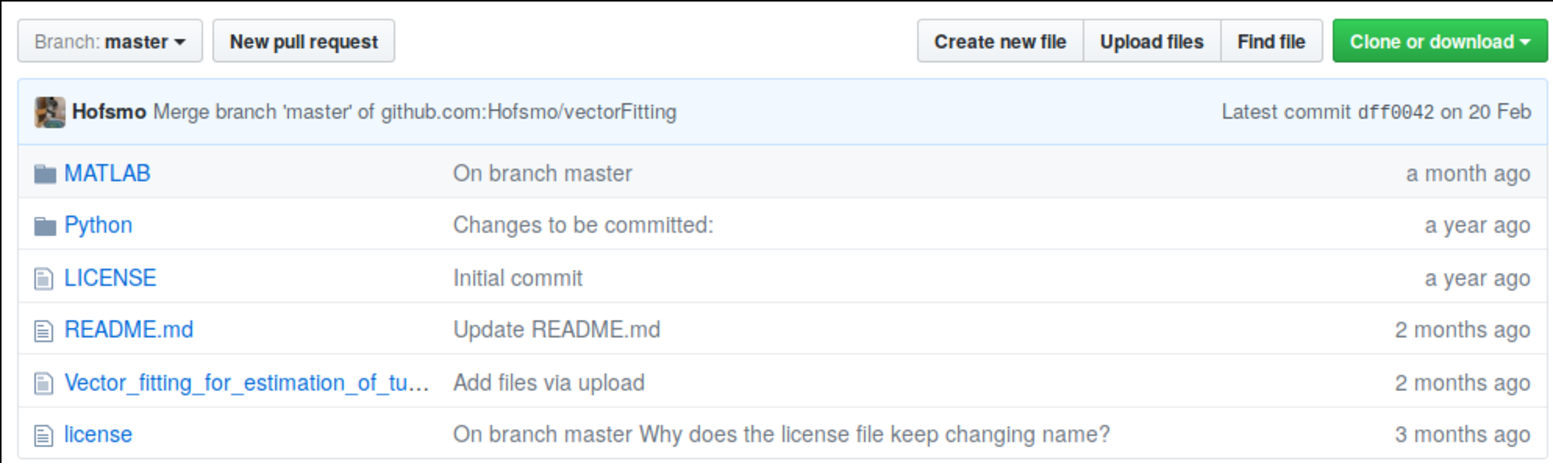
\includegraphics[width=\textwidth]{pictures/git.pdf}
	\end{figure}
\end{frame}
